\documentclass[11pt,a4paper]{article}
\usepackage[margin=1in]{geometry}
\usepackage{graphicx}
\title{Q3\_NETWORK\_MICRO\_2026-03-08\\Scientific Milestone Report}
\author{Science-Chief}
\date{2026-03-08}
\begin{document}
\maketitle

\section*{1. Scope}
This report documents the Q3 micro-network milestone: first graph construction from ERC8004 feedback interactions.

\section*{2. Data Provenance and Purpose}
Data source is the ERC8004 Reputation Registry on Ethereum:
\texttt{0x8004BAa17C55a88189AE136b182e5fdA19dE9b63}, extracted into \texttt{reputation\_newfeedback.csv}.
Purpose: transform event logs into a network object suitable for concentration, centrality, and community analysis.

\section*{3. Extraction and Graph Structure}
From feedback events, we define:
\begin{itemize}
\item Node set A: clients (\texttt{clientAddress})
\item Node set B: agents (\texttt{agentId})
\item Edge: client $\rightarrow$ agent for each feedback event
\item Edge weight: number of repeated feedback events on same pair
\end{itemize}
Then compute weighted in-degree per agent.

\section*{4. Results}
\begin{figure}[htbp]
\centering
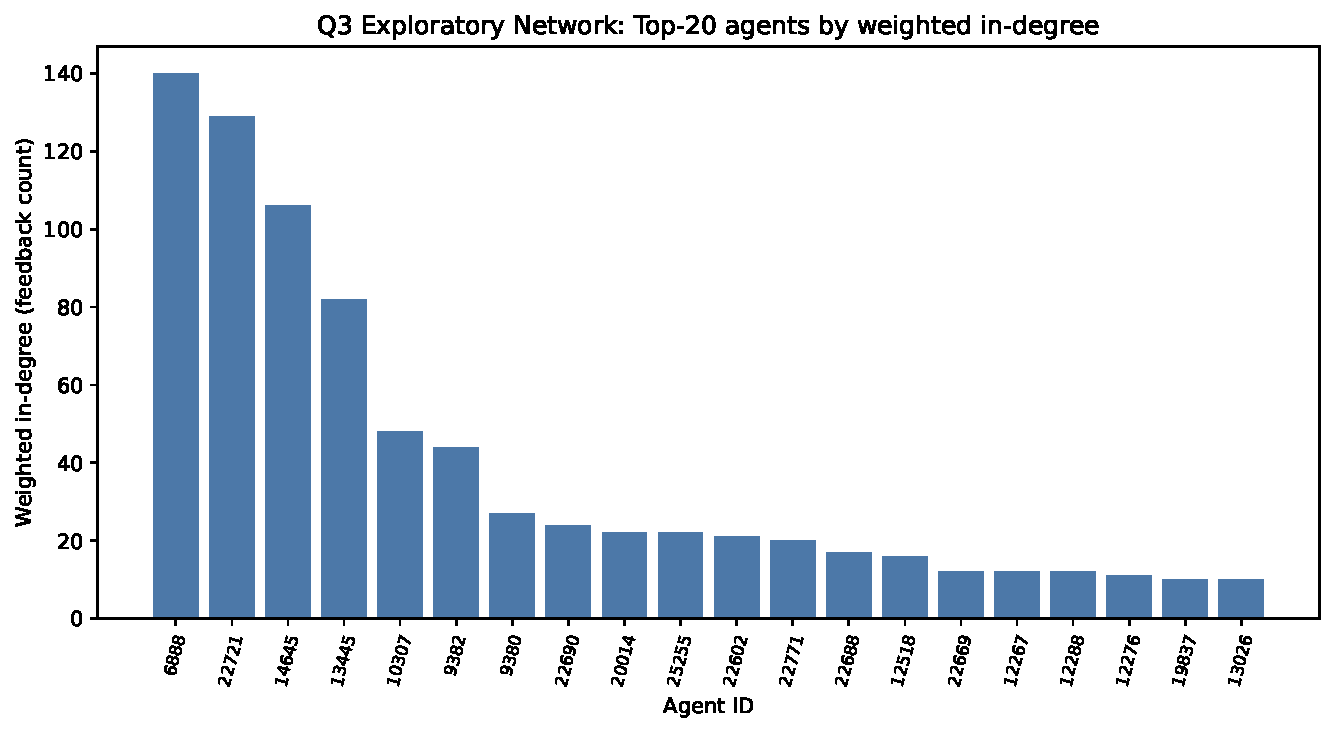
\includegraphics[width=0.9\textwidth]{figures/q3_network_degree_top20.pdf}
\caption{Top-20 agents by weighted in-degree.}
\end{figure}
Snapshot metrics: 1,470 agents with feedback; total weighted in-degree 2,776 (matches event count).

\section*{5. Scientific Interpretation (SC)}
This milestone is a valid network foundation. Degree concentration is visible and consistent with previous concentration findings. However, structural inference is not complete without centrality, community detection, and temporal slicing.

\section*{6. Limitations, Decision, Next}
Current phase is degree-only and static aggregate.
Decision: \textbf{GO internal phase-2 build, HOLD external structural claims}.\
Next: centrality suite, community assignment, temporal windows.

\section*{Appendix: Source Paths}
\textbf{Figures}\\
\begin{itemize}
\item \texttt{workspaces/science-chief/outbox/Reports/Q3\_NETWORK\_MICRO\_2026-03-08/figures/q3\_network\_degree\_top20.pdf}
\end{itemize}
\textbf{Tables}\\
\begin{itemize}
\item \texttt{workspaces/science-chief/outbox/Reports/Q3\_NETWORK\_MICRO\_2026-03-08/tables/q3\_bipartite\_edges\_weighted.csv}
\item \texttt{workspaces/science-chief/outbox/Reports/Q3\_NETWORK\_MICRO\_2026-03-08/tables/q3\_agent\_weighted\_degree.csv}
\item \texttt{workspaces/science-chief/outbox/Reports/Q3\_NETWORK\_MICRO\_2026-03-08/tables/q3\_degree\_top20.csv}
\end{itemize}

\end{document}
